\chapter{Réalisation}
S'appuyant sur un pipeline bien conçu et minutieusement vérifié, la phase de réalisation implique le traitement effectif des données, passant de la théorie à la pratique
\section{Contrôle de qualité}

Avant de procéder à toute analyse, nous avons effectué un contrôle qualité des séquences à l'aide de l'outil FastQC. Cette étape est essentielle pour évaluer la qualité des données brutes et identifier d'éventuels problèmes ou biais qui pourraient affecter les résultats de nos analyses ultérieures.

\subsection*{L'outil}

FastQC est un outil facile à utiliser qui accepte les fichiers de données brutes en format FastQ. Il génère un rapport HTML interactif qui peut être visualisé dans n'importe quel navigateur web. Ce rapport contient une série de graphiques et de tableaux qui aident à comprendre la qualité des données de séquençage \cite{fastqc, fastQC2}.\\

FastQC et à travers son rapport généré, nous permettent d'examiner différentes métriques de qualité, telles que la distribution des scores de qualité, la présence de séquences dupliquées, la présence d'adaptateurs, la qualité de base par position, etc. En examinant ces métriques, nous pouvons déterminer si les données répondent aux critères de qualité requis pour nos analyses et si des étapes supplémentaires, telles que le trimming, sont nécessaires.\\

L'interprétation des résultats de FastQC nécessite une certaine expertise. Chaque module du rapport fournit une "passe" ou un "échec" basé sur les seuils définis pour les données de séquençage de haute qualité. Cependant, un "échec" dans un module ne signifie pas nécessairement que les données sont de mauvaise qualité. Il est important de comprendre le contexte biologique et l'objectif de l'expérience pour interpréter correctement ces résultats.

\subsection*{Le Bloc de commandes}
Ce script, écrit en Bash, automatise l'évaluation de la qualité des données de séquençage en utilisant FastQC. Il est conçu pour améliorer l'efficacité des pipelines bioinformatiques, le script prend deux arguments en entrée : le répertoire d’entrée contenant les fichiers .fastq.gz et le répertoire de sortie où les résultats de l’analyse seront stockés. Si le répertoire de sortie n’existe pas, le script le crée. Ensuite, il utilise la commande find pour rechercher tous les fichiers .fastq.gz dans le répertoire d’entrée. Pour chaque fichier trouvé, il exécute l’outil FastQC, qui analyse la qualité des séquences. Les résultats de l’analyse FastQC sont ensuite enregistrés dans le répertoire de sortie.\\

Après avoir analysé les résultats de FastQC, nous avons identifié plusieurs aspects nécessitant une attention particulière, notamment la présence d'adaptateurs, qui pourraient affecter la fiabilité des données. Ces séquences d'adaptateurs peuvent être éliminées à l'aide d'outils de trimming tels que Cutadapt. Le processus de nettoyage des données va permettre de préparer les données pour les analyses ultérieures.\\

\section{Nettoyage des reads}
Cutadapt représente un outil performant dédié au nettoyage des séquences, capable de filtrer les données selon de multiples paramètres. Fondé sur la transformée de Burrows-Wheeler, il permet une recherche hors ligne de motifs dans un texte. Plusieurs outils sont disponibles pour le trimming des séquences, et nous avons opté pour Cutadapt en raison de sa spécialisation dans le retrait des adaptateurs \cite{martin2011cutadapt}. 

\subsection*{Les métriques de longueur et qualité}
L'outil Cutadapt accepte en paramètre des longueurs maximales et minimales de lectures. Ces paramètres permettent d'exclure toutes les séquences qui ne répondent pas aux normes des miARN. Ainsi, notre longueur maximale est fixée à 30 nucléotides et notre longueur minimale à 15 nucléotides. De cette manière, nous ne conservons que les séquences qui peuvent potentiellement nous être utiles.

\subsection*{L'automatisation}
Le script qui gère l'exécution de cet outil est écrit en Bash. Tout d'abord, il appelle les différents fichiers d'entrée et de sortie des données, ainsi que le fichier CSV contenant les séquences I7/5. Pour permettre à l'utilisateur d'injecter ses propres séquences et éviter les éventuels problèmes et exécutions inutiles, une vérification préalable à l'exécution du trim est effectuée pour garantir que les séquences I7/5 sont conformes aux normes IUPAC. Ensuite, le fichier des données fastaQ est temporairement décompressé avant d'être injecté dans Cutadapt. Pendant tout le traitement, les opérations réalisées par le script sont affichées dans le terminal pour fournir un retour d'information à l'opérateur.

\section{Alignement des séquences}

\subsection*{Accélérer le traitement}
L’alignement des reads sur un génome est une opération a lourde charge computationnelle. Elle implique la recherche de motif (les reads) dans un texte très long (le génome). \\

\noindent BWA\_MEM2 est un algorithme qui associe toutes les techniques les plus modernes pour réduire au maximum le temps de calcul. Voici une liste non exhaustive des « astuces » utilisées ici : 

\begin{itemize}
    \item L’utilisations de la transformée de Burrow Wheeler, cité plusieurs fois dans ce rapport, permet de fortement compresser le texte en regroupant les motifs de ce dernier. 
    \item L’implémentation du parallélisme, il fait référence à la capacité d'exécuter simultanément plusieurs tâches ou instructions en utilisant plusieurs cœurs de processeur sur une même machine. En répartissant la charge de travail les opérations sont réalisées plus rapidement et efficacement.
    \item L’amélioration principale de BWA\_MEM2 sur son prédécesseur BWA est l’implémentation d’une phase de « seeding ». Elle implique d'identifier de courtes correspondances exactes entre un read et le génome de référence. Ces correspondances exactes servent de points de départ pour le processus d'alignement. L'objectif de la phase de « seeding » est d'identifier rapidement des régions potentielles d'alignement, réduisant ainsi l'espace de recherche et la complexité computationnelle des étapes d'alignement suivantes \cite{LISA, MEM2Github}.
\end{itemize} \\ 

\noindent Grace à ces optimisations, cet algorithme est environ deux fois plus rapide que son prédécesseur \cite{bwamem2, BWAimproved}.

\subsection*{La séquence de commandes}
Pour cet outil aussi, le script est écrit en bash, le shell permet une grande simplification du script. Un fichier JSON contenant les accès aux différents fichiers d’input/output est appelé puis les différents génomes de référence sont importés. 

\subsubsection*{L’indexation}
Les index (dans le cadre de l’alignement) sont des prétraitements du texte qui permettent de localiser ultérieurement les reads en son sein. Ces index dans le cadre de BWA\_MEM2 sont la transformée de Burrows-Wheeler, la liste des suffixes ou encore l’index de Ferragina-Manzini (compression de la Burrows-Wheeler).

Ce genre de prétraitement est important dans le cas des méthodes dites « offlines » d’alignement, ces méthodes « offlines » prétraitent le texte à l’inverse des méthodes dites « online » qui prétraitent le pattern. Ici, nous avons des millions de patterns (reads) et seulement quelques textes (génomes de référence) nous pouvons ainsi capitaliser les méthodes offlines pour faciliter les calculs. 

Il se trouve que la génération des indexes peut-être plutôt demandante en ressource. Ainsi dans notre script, elle sera appliquée si et seulement si le génome n’est pas déjà annoté. 
Une fois le génome traité si besoin, tous les reads sont alignés un par un et exportés dans un fichier SAM.
 
\section{Génération des index}

% par la suite Samtools

\begin{quote}
    /TO DO/
\end{quote}

% On parle des outils, comment on a implémenté le script et des potentiels problèmes que l'on a eus. On peut aussi donner un exemple de résultat. 

\section{Identification des miARN}

%  avec ShortStack

\begin{quote}
    /TO DO/
\end{quote}

% On parle des outils, comment on a implémenté le script et des potentiels problèmes que l'on a eus. On peut aussi donner un exemple de résultat. 

\section{Fonctionnalitées du pipeline}
\subsection{Le programme de management}

Le programme \texttt{manager.py} est un gestionnaire de scripts conçu pour faciliter l'exécution de différents fichiers Bash dans le cadre d'une analyse de séquençage ARN. Ce gestionnaire est écrit en Python et utilise le module de logging pour enregistrer les étapes de son exécution, assurant ainsi une traçabilité et une transparence lors de l'analyse des données.\newline

L'une des principales fonctionnalités du gestionnaire est sa capacité à charger et valider un fichier de configuration au format JSON, nommé \texttt{rna\_seq\_config.json}. Ce fichier contient des informations sur les programmes disponibles, leurs chemins d'accès et les ordres dans lesquels ils doivent être exécutés. Le script garantit que les configurations nécessaires sont présentes et valides avant d'exécuter les scripts.\newline

Une fois la configuration chargée et validée, le gestionnaire affiche un menu interactif permettant à l'utilisateur de choisir le script à exécuter. Chaque script est accompagné d'une brève description pour aider l'utilisateur à faire son choix. Le gestionnaire prend également en charge la saisie d'arguments supplémentaires pour certains scripts, ce qui lui confère une flexibilité supplémentaire dans son utilisation.\newline

Lors de l'exécution d'un script, le gestionnaire utilise le module \texttt{subprocess} pour appeler le script Bash correspondant avec les arguments appropriés. Les résultats de chaque exécution sont enregistrés à l'aide du module de logging, permettant à l'utilisateur de suivre le déroulement de l'analyse et de détecter rapidement toute erreur ou problème éventuel.\newline

En cas d'erreur pendant l'exécution du gestionnaire lui-même, toutes les exceptions sont capturées et enregistrées à l'aide du logging, assurant ainsi une gestion robuste des erreurs et une meilleure expérience utilisateur.\newline

En résumé, le script \texttt{manager.py} offre une interface conviviale et robuste pour gérer l'exécution de fichiers Bash dans le cadre d'une analyse de séquençage ARN. Grâce à son utilisation du logging et à sa gestion des exceptions, il garantit une exécution fluide et transparente des scripts, facilitant ainsi le processus d'analyse et de traitement des données.


\subsection{L'utilisation du fichier JSON}
Dans notre programme, nous avons fait le choix d’utiliser un fichier JSON. Il est organisé en un format de données léger et lisible utilisé pour structurer des données. Il facilite l’échange d’informations entre des applications. Son utilité réside dans sa simplicité et sa flexibilité, car il permet de représenter des données structurées de manière hiérarchique à l'aide de paires clé-valeur comme un dictionnaire.

Les fichiers JSON sont largement utilisés pour le stockage de configuration, ainsi, dans notre programme il stocke les paramètres des différents scripts ainsi que leur nom et leur rôle.

\begin{SCfigure}[1][h]
    \centering
    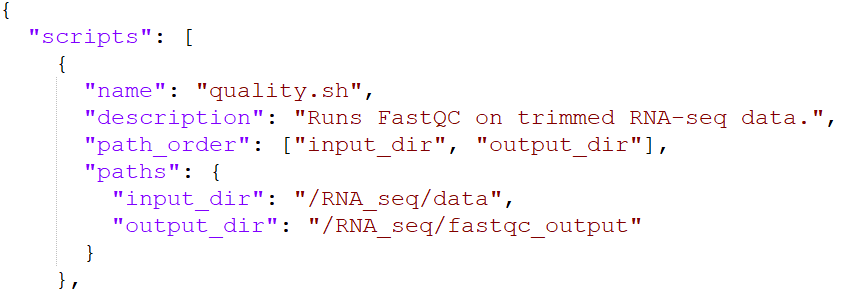
\includegraphics[width=.5\textwidth]{img/exemple_json.PNG}
    \caption{Voici un exemple d’entrée dans notre fichier JSON qui servira à la configuration des scripts.}
    \label{fig:JSON}
\end{SCfigure}


Comme ce format est lisible, il peut facilement être modifié par l’utilisateur et il assure que tous les modules de notre pipeline reçoivent les mêmes informations.


\subsection{Le Logging}

Le logging est une composante cruciale de tout programme informatique, fournissant une traçabilité de l'exécution du programme et facilitant la détection et la résolution des problèmes. Dans le contexte du développement d'une application Python pour l'exécution de commandes Bash, le logging a été intégré de manière à assurer la transparence de l'exécution du programme.\newline

La configuration du logging est définie au début du script, spécifiant le niveau de logging sur INFO et le format des messages. Par exemple, voici une configuration de logging typique :

\begin{lstlisting}[language=Python, breaklines=true]
logging.basicConfig(level=logging.INFO, format='%(asctime)s - %(levelname)s - %(message)s')
\end{lstlisting}

Dans le script fourni, le logging est utilisé pour enregistrer des messages d'importance INFO et supérieure, fournissant ainsi une vue détaillée du déroulement du programme. Par exemple, des messages INFO sont utilisés pour signaler le démarrage et la fin de l'exécution des scripts, ainsi que pour afficher les arguments utilisés lors de l'exécution. Voici un exemple de message INFO enregistré pendant l'exécution du script :

\begin{lstlisting}[language=Python, breaklines=true]
2024-05-12 15:30:00 - INFO - Running script: /path/to/script.sh with arguments: [arg1, arg2, arg3]
\end{lstlisting}

En outre, le logging est également utilisé pour enregistrer les erreurs survenues pendant l'exécution du programme. Les messages d'erreur sont enregistrés avec un niveau de journalisation ERROR, permettant ainsi de les identifier facilement parmi les messages d'état normaux. Par exemple, voici un exemple de message d'erreur enregistré lorsqu'une erreur se produit pendant l'exécution d'un script :

\begin{lstlisting}[language=Python, breaklines=true]
2024-05-12 15:35:00 - ERROR - Failed to execute /path/to/script.sh: Return code 1
\end{lstlisting}

Enfin, le logging est utilisé pour signaler des situations potentiellement problématiques qui ne sont pas des erreurs graves. Ces messages sont enregistrés avec un niveau de journalisation WARNING. Par exemple, voici un exemple de message WARNING enregistré lorsque l'utilisateur saisit une entrée invalide lors du choix d'un script à exécuter :

\begin{lstlisting}[language=Python, breaklines=true]
2024-05-12 15:40:00 - WARNING - Invalid choice, please choose a number between 1 and 4
\end{lstlisting}

L'ensemble de ces messages de logging fournit une traçabilité complète de l'exécution du programme, facilitant ainsi la détection et la résolution des problèmes éventuels. En enregistrant les messages dans un format structuré, il devient également plus facile d'analyser les journaux et d'extraire des informations importantes sur le fonctionnement du programme.

\section{Le fichier ReadMe}

% must add a line or two about ReadMe

\section{Utilisation de Git}

Pour faciliter notre travail collaboratif et assurer une gestion efficace de notre code source, nous avons opté pour l'utilisation de GitHub comme plateforme principale. Les fonctionnalités de contrôle de version de Git ont permis aux membres de l’équipe de travailler ensemble et de suivre les modifications apportées au code tout au long du projet. L'ensemble des scripts, ainsi que le cahier des charges et le rapport en format TeX, ont été déposés dans le répertoire GitHub dédié au projet (https://github.com/Lucien-Piat/RNA-Seq-Fusarium). De plus, GitHub offre à l'ensemble de l'équipe et aux clients un accès pratique et sécurisé au code. En accordant aux clients l'accès au dépôt, ils peuvent non seulement exécuter le programme, mais également examiner le code source lui-même à tout moment.
